\pagestyle{fancy}
\renewcommand{\theUnit}{5}
\ifthenelse{\isundefined{\UnitPageNumbers}}{}{\setcounter{page}{1}}
\rhead{Chapter \theUnit: Bootstrap Confidence Intervals}
\lhead{Math 3382: Statistical Theory}
%\lhead{
\includegraphics[width=1.25cm]{CUDenver-Logo.png}}
\rfoot{\mypage}
\cfoot{
\includegraphics[width=2.25cm]{CUDenver-Logo-coverpage.png}}
\lfoot{Adam Spiegler}
\fancypagestyle{firstfooter}{\footskip = 50pt}
\renewcommand{\footrulewidth}{.4pt}
%%%%%%%%%%%%%%%%%%%%%%%%%%%
\vspace*{-20pt} \thispagestyle{firstfooter}


%\begin{tasks}[counter-format = {(tsk[a])},label-offset = {0.8em},label-format = {\color{black}\bfseries}](2)


\pagebegin{Bootstrap Interval Estimates}

Usually when estimating an unknown population parameter, we give an \textbf{\colorb{interval estimate}} that gives range of plausible values for the parameter by accounting for the uncertainty due to the variability in sampling.


\begin{center}
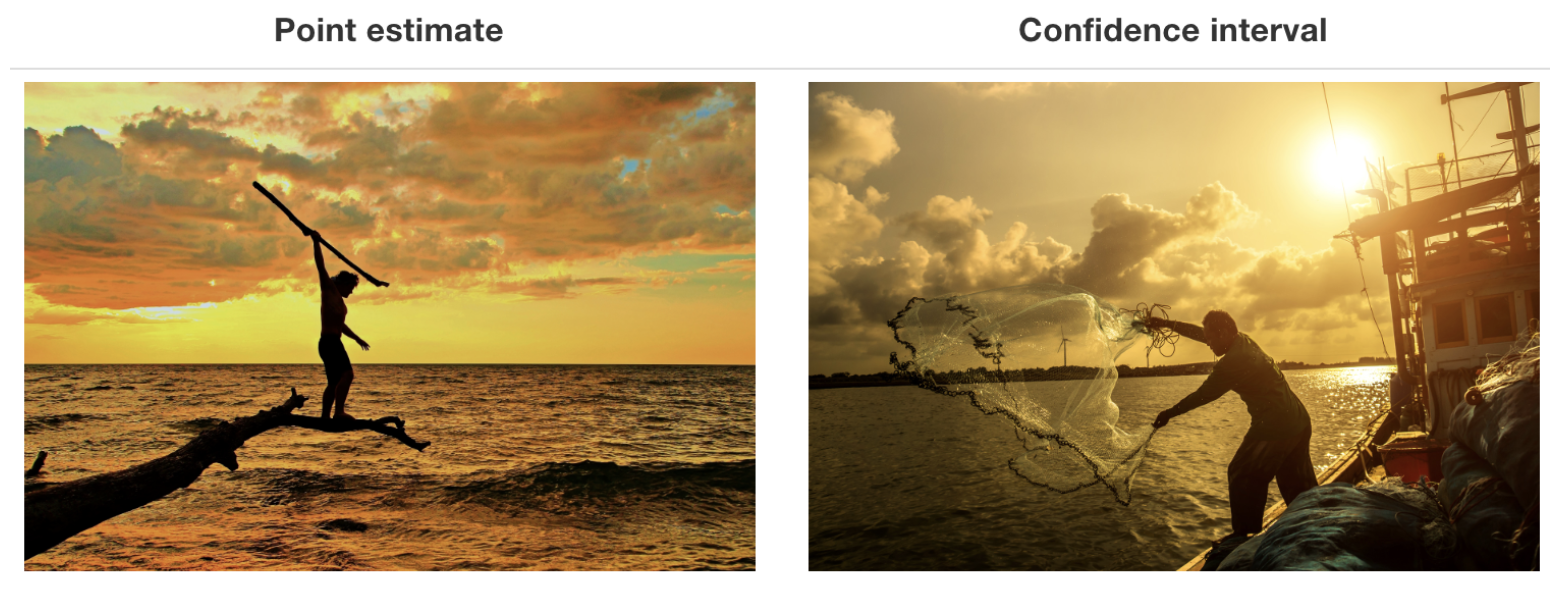
\includegraphics[width=0.75\tw]{12/fig-fishing.png}
\end{center}

\bbox
The interval between the $2.5$ and $97.5$ percentiles of the bootstrap distribution of a statistic is a \textbf{\colorb{95\% bootstrap percentile confidence interval}} for the corresponding parameter.

\bi
\ii If most of the sample statistics are located in a certain interval of the bootstrap distribution, it seems plausible the true value of the parameter is in this interval!
\ii We would say we are 95\% confident that the interval contains the actual value of  the population parameter.
\ei
\ebox

\bb
\ii We return the bootstrap distribution we created to approximate the sampling distribution for the mean arsenic level of groundwater in Bangladesh. See the R Markdown file that goes along with this case study to answer the questions below.
\bb
\ii Find bootstrap percentiles and give a 95\% bootstrap percentile confidence interval for the mean arsenic level in groundwater in Bangladesh. \vfill 

\ii Interpret the practical meaning of the interval. \vfill

\ii Sometimes it is nice to describe the interval as a value plus or minus some margin of error. Recall with normal distributions, approximately 95\% of the data is within 2 standard deviations of center of the distribution.  Construct a symmetric 95\% bootstrap confidence interval for the mean arsenic level.  \vfill
\ee

\clearpage

\ii We return to the mean weight of newborns in North Carolina from earlier. Answer the questions below assuming the population is all newborns in North Carolina in 2004 (which is unknown), and we have one large random sample size $n=1009$ in the dataset \textit{\textbf{\colorg{NCBirths2004}}}. See the R Markdown file that goes along with this case study to answer the questions below.

\bb
\ii Give a 95\% bootstrap percentile confidence interval for the mean weight of babies born in North Carolina in 2004.\vfill %See \textbf{NCBirths.R}.

\ii Give a 90\% bootstrap percentile confidence interval for the mean weight of babies born in North Carolina in 2004. \label{q:90per} \vfill

\ii Interpret the practical meaning of your 90\% bootstrap percentile confidence interval in question \ref{q:90per}. \vfill

\ii When we decreased the confidence level, what happened to the confidence interval estimate? \vfill
\ee
\ee


\clearpage

\pagebegin{Two-Sample Bootstraps}

\bbox
Given independent samples of sizes $m$ and $n$ from two populations:
\bi
\ii Draw a resample of size $m$ with replacement from the first sample.
\ii Draw a resample of size $n$ with replacement from the second sample.
\ii Compute a statistic that compares the two groups such as a difference or ratio of two means.
\ii Repeat resampling many times over.
\ii Construct a bootstrap distribution of the statistic.
\ei
\ebox

\bb[resume]
\ii What is the difference between the length of commercials on basic cable channels and on extended cable channels? The table
shows the total number of minutes devoted to commercials during randomly selected half-hour periods on basic and extended cable TV channels\footnote{Rodgers and Robinson (2004)}. See the R Markdown file that goes along with this case study to answer the questions below.

\begin{center}
\begin{tabular}{l|cccccccccccc}
\hline
Basic & $7$& $10$ & $10.6$ & $10.2$ & $8.6$ & $7.6$ & $8.2$ & $10.4$ & $11.0$ & $8.5$\\
Extended & $3.4$ & $7.8$ & $9.4$ & $4.7$ & $5.4$ & $7.6$ & $5.0$ & $8.0$ & $7.8$ & $9.6$ & $6.2$ & $8.1$\\
\hline
\end{tabular}
\end{center}

\bb
\ii Use exploratory data analysis to compare the two groups. \vfill

%\clearpage

%times.Basic $<-$ c(7, 10, 10.6, 10.2, 8.6, 7.6, 8.2, 10.4, 11.0, 8.5)\\
%times.Ext $<-$ c(3.4, 7.8, 9.4, 4.7, 5.4, 7.6, 5.0, 8.0, 7.8, 9.6, 6.2, 8.1)\\

%\begin{multicols}{2}

%hist(times.Basic) \\
%hist(times.Ext)\\
%boxplot(times.Basic, times.Ext, \\
% \indent \ \ \ \ \ \ \ \ \ \ \ \ \ \ \ \ \ names = c("Basic", "Extended"))\\
%\\
%mean(times.Basic)\\
%sd(times.Basic)\\
%n.Basic $<-$ length(times.Basic)\\
%\\
%mean(times.Ext)\\
%sd(times.Ext)\\
%n.Ext $<-$ length(times.Ext)\\
%observed $<-$ mean(times.Basic) - mean(times.Ext)\\
%observed\\

%\columnbreak

%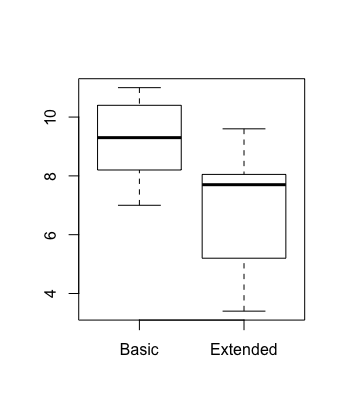
\includegraphics[width=0.4\tw]{12/fig-cable-box.png}
%\[ \mbox{difference in means} = 9.21 - 6.917  =  2.293\]
%\end{multicols}

\ii Generate one possible bootstrap resample (from each sample). \vfill

\ii Give a  \textbf{90\% bootstrap percentile confidence interval}  to estimate the difference between the length of commercial times. \vfill

\ii Interpret the practical meaning of your interval estimate . \vfill
\ee
\ee

%\begin{multicols}{2}
%N $<- 10^4$\\
%times.diff.mean $<-$ numeric(N)\\
%\\
%for (i in 1:N)\\
%$\left\{ \right.$\\
%\indent \ \ \ \ \ \   Basic.boot $<-$ sample(times.Basic,  \\
%\indent \ \ \ \ \ \ \ \ \ \ \ \ \ \ \ \ \ n.Basic, replace=TRUE)\\
% \indent \ \ \ \ \ \    Ext.boot $<-$ sample(times.Ext, \\
% \indent \ \ \ \ \ \ \ \ \ \ \ \ \ \ \ \ \  n.Ext, replace=TRUE)\\
%\indent \ \ \ \ \ \  times.diff.mean[i] $<-$  mean(Basic.boot)-mean(Ext.boot)\\
%$\left. \right\}$\\
%\\
%lower $<-$ quantile(times.diff.mean, probs = 0.05)\\
%upper $<-$ quantile(times.diff.mean, probs = 0.95)\\
%\\
%hist(times.diff.mean)\\
%abline(v = observed, col = "red", lwd = 2, lty = 2)\\
%abline(v = lower, col = "blue", lwd = 2, lty = 2)\\
%abline(v = upper, col = "blue", lwd = 2, lty = 2)
%abline(v = mean(times.diff.mean), col = "green", lwd = 2, lty = 2)
%\columnbreak

%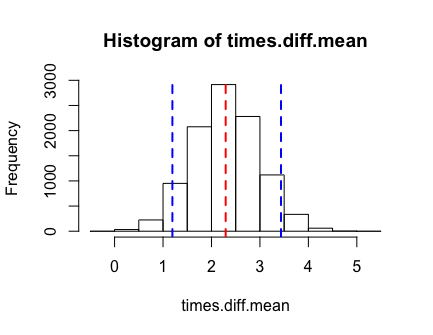
\includegraphics[width=0.5\tw]{12/fig-cable-boot.png}

%\[ \hat{\theta} = \bar{x}_{\rm{basic}} - \bar{x}_{\rm{Ext}} = 2.299 , \ \ \  \hat{\mbox{SE}} = 0.680 \]
%\begin{center} 90\% Bootstrap CI: $1.193$ to $3.435$ minutes \end{center}
%\end{multicols}

\clearpage

\pagebegin{Matched Pair Samples}

\begin{multicols}{2}

In the 2008 Olympics there was a lot of controversy over new swimsuits that possibly provided an unfair advantage to swimmers which led to new international rules regarding swimsuit materials and coverage. Can a swimsuit really make a swimmer faster?

\bigskip

A study\footnote{de Lucas, Balidan, Neiva, Grecco, and Denadai. ``The effects of wetsuits on physiological and biomechanical indices during swimming'', \textit{Journal of Science and Medicine in Sport}} tested whether wearing wetsuits influences swimming velocity. Twelve competitive swimmers swam 1500 meters at maximum speed twice each. Once wearing a wetsuit and once wearing a regular bathing suit. The order of the trials was randomized. Each time, the maximum velocity in meters/sec of the swimmer was recorded.

\columnbreak

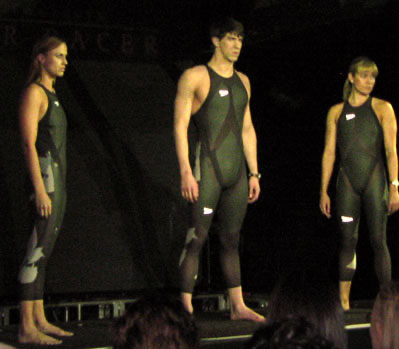
\includegraphics[width=0.35\tw]{12/fig-phelps.jpg}

\end{multicols}

\vspace{0.5in}

\begin{tabular}{|l||c|c|c|c|c|c|c|c|c|c|c|c|}
Swimmer & 1 & 2 & 3 & 4 & 5 & 6 & 7 & 8 & 9 & 10 & 11 & 12 \\
\hline
Wetsuit & $1.57$ & $1.47$ & $1.42$ & $1.35$ & $1.22$ & $1.75$ & $1.64$ & $1.57$ & $1.56$ & $1.53$ & $1.49$ & $1.51$ \\
No Wetsuit & $1.49$ & $1.37$ & $1.35$ & $1.27$ & $1.12$ & $1.64$ & $1.59$ & $1.52$ & $1.50$ & $1.45$ & $1.44$ & $1.41$ \\
\hline
Difference & $0.08$ &  $0.10$ &  $0.07$ &  $0.08$ &  $0.10$ & $0.11$ & $0.05$ & $0.05$ & $0.06$ & $0.08$ & $0.05$ &  $0.10$
\end{tabular}

\vspace{0.5in}

\bbox
Notice the structure of the data above is different from sampling from two independent populations.
\bi
\ii Each sample consists of one reading from each of the same 12 people.
\ii There is a very natural way to match each value from one sample to exactly one value from the other sample.
\ii The data consists of 12 different \textbf{\colorb{matched pairs}}.
\ii For each pair, we can associate a single value, such as a difference in the two velocities.
\ii We can estimate the value of some statistic (such as the mean) to summarize the matched pair sample.
\ei
\ebox

\clearpage

\pagebegin{Matched Pair Bootstrap Distributions}

\bbox
Given matched samples each of size $n$:
\bi
\ii For each pair calculate the difference.
\ii Consider the collection of $n$ differences as your original sample.
\ii Draw a resample of size $n$ with replacement from the sample of differences. Compute the relevant statistic.
\ii Repeat this many times.
\ii Construct the bootstrap distribution of the statistic.
\ei
\ebox


\bb[resume]
\ii The researchers want to construct a 99\% bootstrap percentile confidence interval to estimate the mean difference in the velocities with the two different types of swimsuits. See the R Markdown file that goes along with this case study to answer the questions below.

\bb
\ii Generate one possible bootstrap resample using this process. \vfill


\ii Construct a 99\% bootstrap percentile confidence interval to estimate this difference. \vfill

\ii Interpret the practical meaning of your interval estimate. \vfill
\ee
\ee

%\begin{multicols}{2}
%Diff $<-$ wetsuit - none \\
%observed $<-$mean(Diff) \\ 
%observed\\
%n $<-$ length(Diff)\\
%\\
%N $<- 10^5$\\
%boot.diff $<-$ numeric(N)\\
%\\
%for (i in 1:N)\\
%$\left\{ \right.$\\
%\indent \ \ \ \ \ \  result $<-$ sample(Diff, n, replace = TRUE)\\
%\indent \ \ \ \ \ \  boot.diff[i] $<-$ mean(result)\\
%$\left. \right\}$\\
%\\
%lower $<-$ quantile(boot.diff, probs = 0.025)\\
%upper $<-$ quantile(boot.diff, probs = 0.975)\\
%lower\\
%upper\\

%hist(boot.diff, xlab = "Difference", \\
 %\indent \ \ \ \ \ \   main = "Bootstrap Distribution")\\
%abline(v = observed, col = "red", lwd = 2, lty = 2)\\
%abline(v = lower, col = "blue", lwd = 2, lty = 2)\\
%abline(v = upper, col = "blue", lwd = 2, lty = 2)

%\columnbreak

%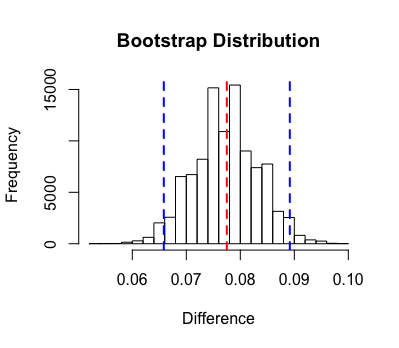
\includegraphics[width=0.5\tw]{12/fig-swim-boot.png}

%\[ \hat{\theta} = \bar{x}_{\rm{diff}} = 0.0774 , \ \ \ \hat{\mbox{SE}} = 0.006 \]
%\begin{center} 95\% Bootstrap CI: $0.066$ to $0.089$ m/sec \end{center}
%\end{multicols}

